\section{Experiment}
In diesem Kapitel werden die Sicherheitsgefahren und -risiken von IoT-Geräten
demonstriert.  Dafür wurde eine Raspberry Pi-Sicherheitskamera mithilfe der
Open-Source-Bibliothek \textit{pi-aREST} \cite{piarestgtihub, piarestnpm}
entwickelt. Die Sicherheitskamera sendet mithilfe von \textit{pi-aREST} in
einem festgelegten Zeitintervall ein Bild, des überwachten Bereichs, an ein
externes System. Die Entscheidung \textit{pi-aREST} als Bibliothek für die
Entwicklung des IoT-Gerätes zu verwenden, hatte mehrere Gründe.  Ein Grund war,
dass die Bibliothek im speziellen für die Arbeit mit dem Raspberry Pi
entwickelt wurde und eine direkte Implementierung für das Erstellen von Bildern
mithilfe einer angeschlossenen Kamera enthält. Außerdem ist der Quellcode
Open-Source, wodurch die Bibliothek einfacher untersucht und auf potentielle
Sicherheitsrisiken überprüft werden kann \cite{piarestgtihub}. Der Entwickler
der Bibliothek bietet zudem einen eigenen Überwachungs- und Kontroll-Service,
für die mit der Bibliothek entwickelten IoT-Geräte, an. Wodurch die
Untersuchung der möglichen Sicherheitsprobleme anhand von realistischen
Szenarien demonstriert werden kann \cite{arestservice}.

\begin{figure}[t]
  \centerline{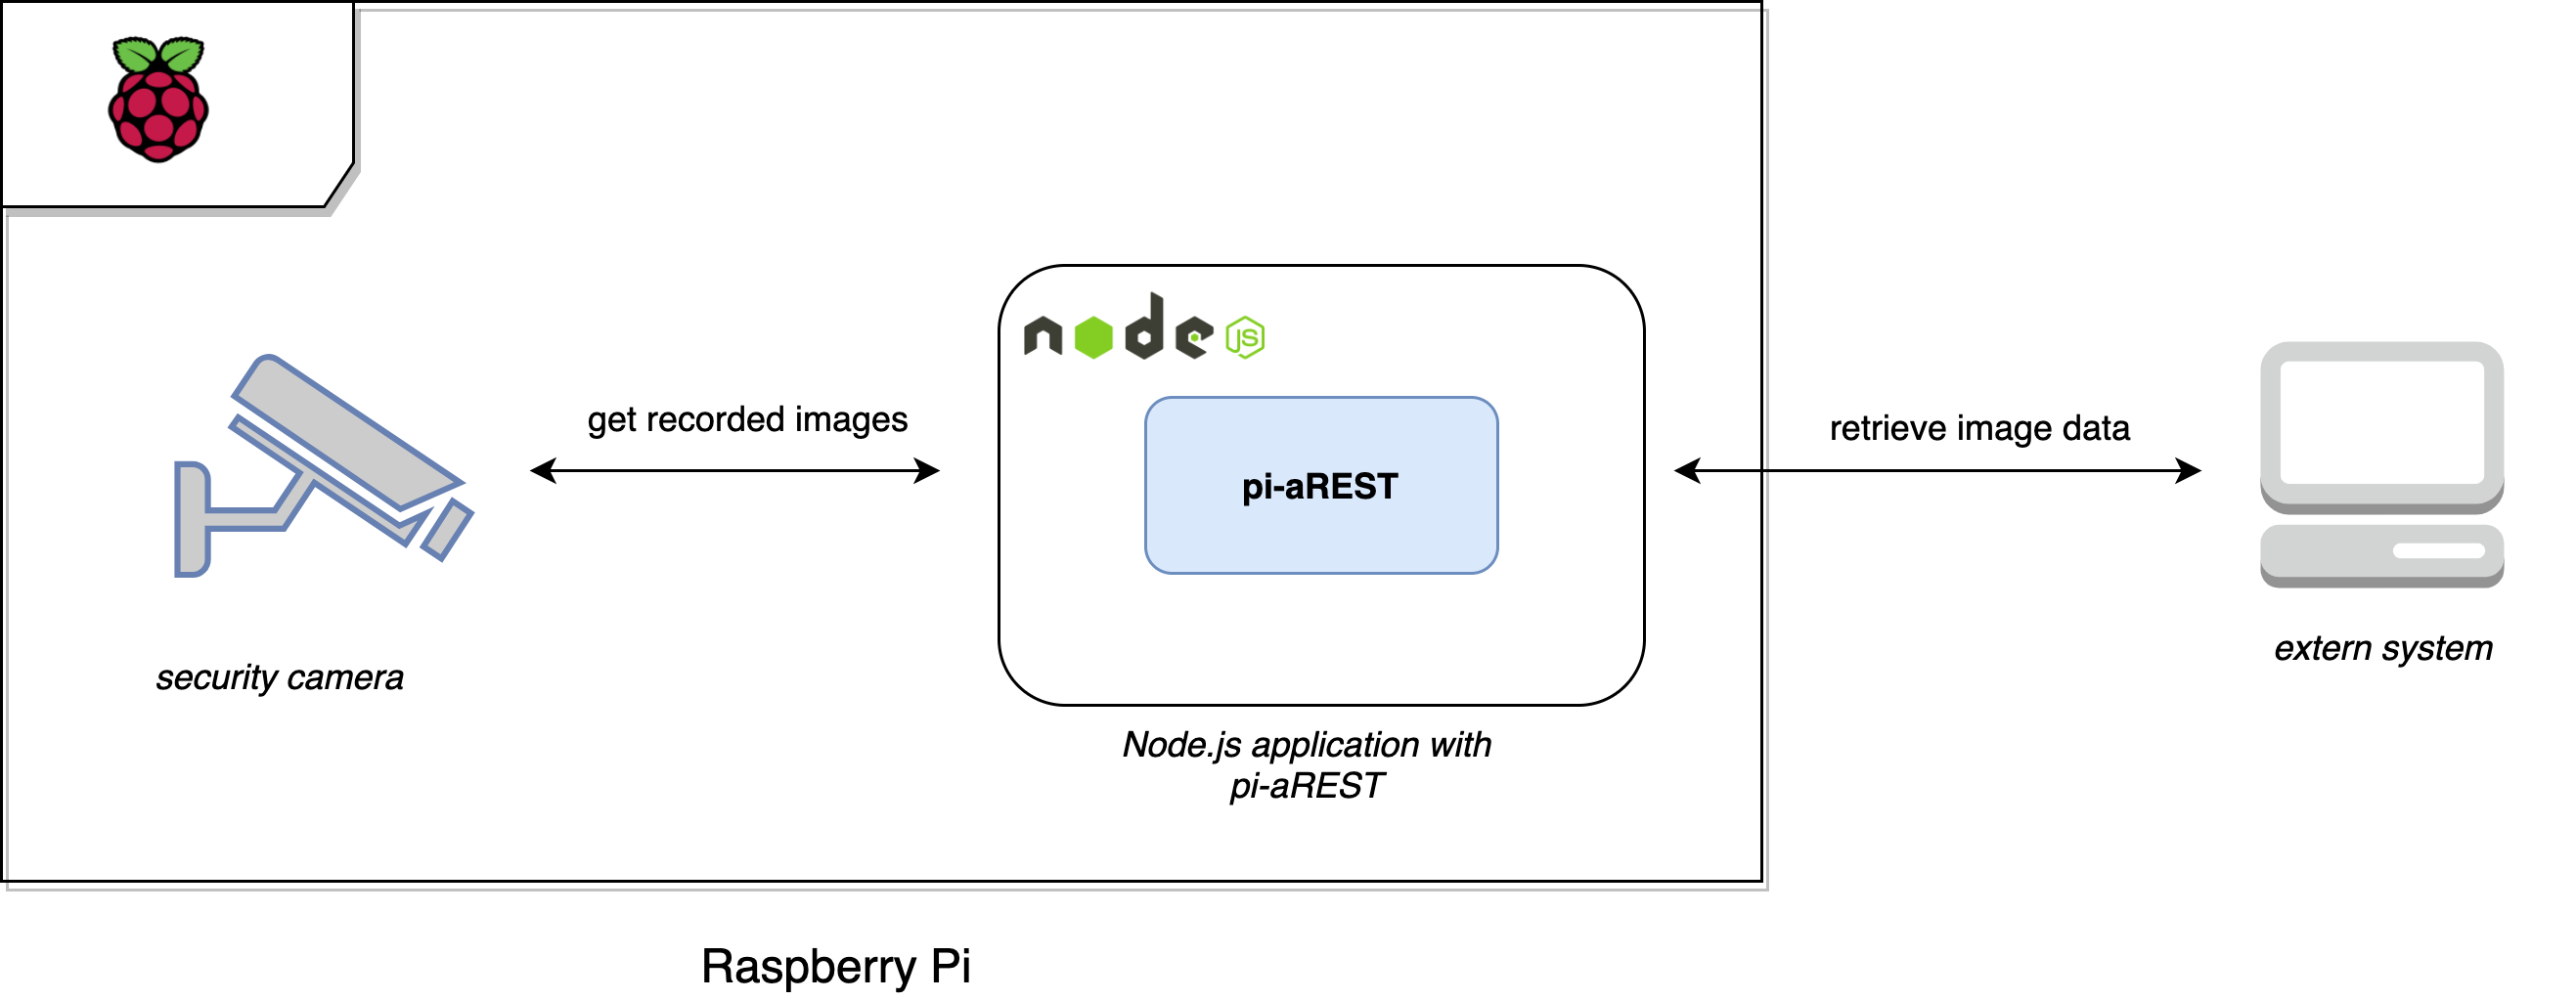
\includegraphics[width=250px]{images/raspberry_architecture}}
  \caption{Sicherheitskamera-Architektur}
  \label{fig:arch-raspberrypi}
\end{figure}

\subsection{pi-aREST}
\textit{pi-aREST} ist eine Bibliothek für die JavaScript-Laufzeitumgebung
\textit{Node.js} \cite{node}, welche mithilfe des Package-Managers \textit{npm}
\cite{piarestnpm} in eine Node-Anwendung importiert werden kann. Durch das
Einbinden von \textit{pi-aREST} in eine eigene Node-Anwendung werden
Schnittstellen zur Kommunikation mit anderen Systemen und Geräten geöffnet. Der
Datenaustausch erfolgt dabei mithilfe der Protokolle \textit{HTTP} und
\textit{MQTT} und kann sowohl in lokalen Netzwerken, als auch im Internet
stattfinden \cite{piarestgtihub}.

\subsubsection{HTTP-Server}
Nachdem Ausführen der Node-Anwendung mit der importierten Bibliothek, startet \textit{pi-aREST} einen 
\textit{express} HTTP-Server auf dem IoT-Gerät zum Bereitstellen einer REST-API. Die API besitzt
verschiedene Endpunkte, welche entweder innerhalb des Netzwerkes oder aus dem Internet aufgerufen werden
können.  \cite{piarestgtihub}

\begin{table*}[t]
  \centering
  \label{tab:security-threats}
  \begin{tabularx}{\textwidth}{lX}
    \textbf{Endpunkt} & \textbf{Aufgabe}\\
    \hline
    \textbf{/} & Liest die allgemeinen Raspberry Pi-Informationen (ID, Name) und weitere
		    Metadaten, die in einem JavaScript Objekt festgehalten sind, aus und gibt 
		   diese zurück  \\

    \textbf{/:variable} & Anhand des übergebenen Parameters \textit{variable} wird in einem 
				JavaScript-Objekt, dass Metadaten zum Raspberry Pi enthält, überprüft, ob dieses ein
				Attribut mit diesem Namen enthält. Wenn dies der Fall ist, wird es an den
				Anfragenden zurückgegebenen. Unter JavaScript kann das Attribut auch
				eine Funktion sein, falls dies der Fall ist, wird diese ausgeführt und das 
				Ergebnis zurückgegeben. \\

    \textbf{/camera/snapshot} & Erstellt ein Bild durch die am Raspberry PI angeschlossene Kamera 
					     und hinterlegt dieses im Dateisystem.  \\

    \textbf{/:command/:pin} & Liest den Status des über den Parameter \textit{pin} angegebenen digitalen
					Pins aus und sendet diesen Status zurück.   \\

    \textbf{/digital/:pin/:state} & Ermöglicht das Setzten eines Status zu einem Pin, indem über den Parameter 
					\textit{pin} der zu aktualisierende Pin ausgewählt wird und der Parameter
					\textit{state} den neuen Status festlegt.  \\
  \end{tabularx}
  \caption{Endpunkte eines \textit{pi-aREST}-HTTP-Servers \cite{piarestgtihub}}
\end{table*}

\subsubsection{MQTT-Client}
\textit{Message Queuing Telemetry Transport (MQTT)} ist ein Open-Source
Kommunikationsprotokoll auf der Anwendungsebene. Das Protokoll zeichnet sich
durch ressourcensparende Datenpakete mit einem geringen Overhead aus, wodurch
es bspw. oftmals in der Kommunikation zwischen IoT-Geräten (M2M) eingesetzt
wird. Das Protokoll basiert auf der Publish/Subscribe-Architektur. So nehmen
Clients die Rollen eines \textit{Publisher (Sender)} oder \textit{Subscriber
(Em- pfänger)} ein und kommunizieren über den sogenannten \textit{Broker}
miteinander. \cite{mqtt, wong20man}

\paragraph{Publisher} 
Dieser Client sendet Nachrichten an einen \textit{Broker}, wobei die
übersendeten Nachrichten eine spezielle \textit{Topic (Bezeichner)} enthalten.
Die übergebene \textit{Topic} ist wichtig für das Weiterleiten der Nachrichten
an andere Clients. \cite{mqtt, wong20man}

\paragraph{Subscriber} 
Im Gegenteil zum \textit{Publisher} sendet der \textit{Subscriber} keine
Nachrichten an \textit{Broker}, sondern abonniert \textit{(subscriped}) sich
beim \textit{Broker} für eine bestimmtes \textit{Topic}.  Wenn ein
\textit{Publisher} eine Nachricht mit dem abonnierten \textit{Topic} an den
\textit{Broker} sendet, erhalten alle \textit{Subscriber} dieses
\textit{Topics} die Nachricht \cite{mqtt, wong20man}.

\paragraph{Broker} 
Die Funktionalität des \textit{Brokers} wurde bereits teilweise bei den anderen
Protokoll-Teilnehmern beschrieben. Seine Hauptaufgabe ist das Steuern des
Datenverkehrs zwischen den verschiedenen Clients.  So nimmt dieser die
Nachrichten der \textit{Publisher} an und sendet diese nur an die, für das
\textit{Topic} abonnierte, \textit{Subscriber} \cite{mqtt, wong20man}.

Beim Ausführen der Node-Anwendung mit \textit{pi-aREST} verbindet sich das
IoT-Gerät als Publisher-Client mit einem MQTT-Broker über den Port 1883. Die
Broker-Adresse wird von der Node-Anwendung vorgegeben.  \textit{pi-aREST}
sendet daraufhin die Verbindungsanfrage an den Broker. Das IoT-Gerät sendet
nach dem erfolgreichen Verbindungsaufbau in einem regelmäßigen Zeitintervall
die Daten, in im Falle des Experimentes die Überwachungsbilder, mit einem
speziellen Topic an den Broker \cite{piarestgtihub}.

\begin{figure}[htbp]
  \centering
  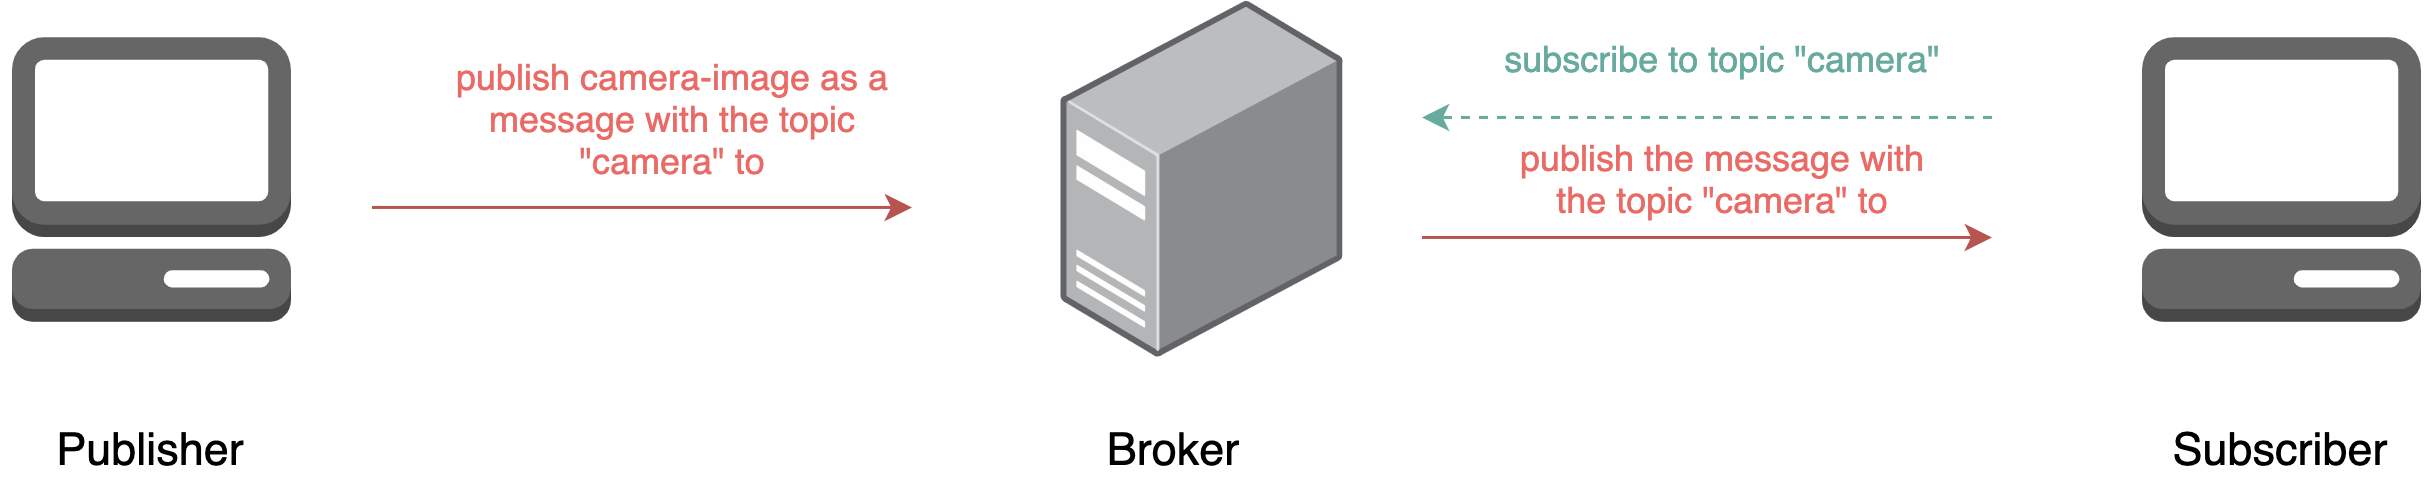
\includegraphics[width=250px]{images/mqtt.png}
  \caption{MQTT-Architektur für die Node-Anwendung \cite{mqtt}}
  \label{fig:arch-mqtt}
\end{figure}

